% !TEX program = pdflatex
% Statistical Pharmacology via Kakutani Dichotomy VII
% Companion computations: benchmark_allosteric_protein.py, code/paper07_compute_tables.py
\documentclass[11pt,reqno]{amsart}

\usepackage[T1]{fontenc}
\usepackage[utf8]{inputenc}
\usepackage{lmodern}
\usepackage[a4paper,margin=27mm]{geometry}
\usepackage{amsmath,amssymb,amsthm,mathtools}
\usepackage{booktabs}
\usepackage{graphicx}
\graphicspath{{./}{../figures/}}
\usepackage{array}
\usepackage{microtype}
\usepackage{enumitem}
\usepackage{xcolor}
\usepackage[colorlinks=true,linkcolor=blue!60!black,citecolor=blue!60!black,urlcolor=blue!60!black]{hyperref}

\theoremstyle{plain}
\newtheorem{theorem}{Theorem}[section]
\newtheorem{lemma}[theorem]{Lemma}
\newtheorem{proposition}[theorem]{Proposition}
\newtheorem{corollary}[theorem]{Corollary}
\theoremstyle{definition}
\newtheorem{definition}[theorem]{Definition}
\theoremstyle{remark}
\newtheorem{remark}[theorem]{Remark}
\numberwithin{equation}{section}

\newcommand{\dd}{\mathrm{d}}
\newcommand{\EE}{\mathbb{E}}
\newcommand{\DCKI}{\Delta\mathrm{CKI}}
\newcommand{\pkg}{\texttt{kakutani\_pharma}}

\renewcommand{\abstractname}{Summary}
\setlength{\emergencystretch}{2em}

\title[Statistical pharmacology via Kakutani dichotomy VII]{Statistical Pharmacology via Kakutani Dichotomy VII:\\ The \texttt{kakutani\_pharma} Pipeline, Ledoit--Wolf Regularized CKI, Split-Trajectory Null Subtraction, and Shell-Scaling Exponents in Multi-Domain Allostery}

\author[Z. Chen]{Zhengyi Chen}
\address{Guangxi Key Laboratory of Drug Discovery and Optimization, School of Pharmacy, Guilin Medical University, Guilin 541199, P.~R. China}
\email{chenzhengyi@glmc.edu.cn}

\author[R. Chen]{Ruqing Chen}
\address{GUT Geoservice Inc., Montreal, Qu\'ebec, Canada}
\email{ruqing@hotmail.com}

\thanks{DOI: \href{https://doi.org/10.5281/zenodo.23039869}{10.5281/zenodo.23039869}.\newline Sources, code and data: \url{https://github.com/Ruqing1963/kakutani-statistical-pharmacology-VII}. Papers I--VI of the series are \cite{ChenChen2026I,ChenChen2026II,ChenChen2026III,ChenChen2026IV,ChenChen2026V,ChenChen2026VI}; the underlying monograph is \cite{Chen2026}.}
\thanks{This project was supported by the National Natural Science Foundation of China (No.~22464010), the Guangxi Natural Science Foundation of China (No.~2025GXNSFAA069294), and the 2025 Bagui Youth Top Talent Project.}
\date{29 September 2026}

\subjclass[2020]{Primary 62H12, 92C40; Secondary 62F40, 62M10, 52C25, 15A15}
\keywords{Kakutani index, Bhattacharyya distance, Ledoit--Wolf shrinkage, high-dimensional covariance, block bootstrap, split-trajectory null, elastic network model, infinitesimal rigidity, allostery, molecular dynamics}

\begin{document}

\begin{abstract}
Papers I--VI studied Kakutani indices of idealised infinite conformational ensembles. This paper turns them into estimators for finite trajectories, implemented in the open Python package \pkg{}. The package combines dihedral metastable states, contact networks and joint mass-weighted superposition with a Laplace-smoothed first-order index (DKI), a second-order index (CKI) regularised by analytical Ledoit--Wolf shrinkage, a spectral fingerprint, and pocket-centred shell scaling. Finite sampling raises three obstacles: rigid-body motion must be removed jointly, the sample covariance is singular (CKI $=\infty$), and the index carries a large positive bias. Each is treated by a result. Proposition~\ref{prop:rigidity} gives the zero-mode count of an elastic network: two rigid halves joined by $c$ springs have $\dim\ker H=12-c$, which explains the $11$ zero modes of a first benchmark geometry; the compact four-domain geometry A1-1$|$S-1$|$S-2$|$A1-2 has exactly $6$. Theorem~\ref{thm:lw} shows that Ledoit--Wolf shrinkage is positive definite for any number of frames and preserves the exact decomposition $\mathrm{CKI}=D_{\mathrm{mean}}+D_{\mathrm{comm}}+D_{\mathrm{rot}}$ into nonnegative terms. With $200$ frames in $360$ dimensions the sample index is infinite, and the shrunk index is $66.18$ ($\delta=0.157$); the implementation matches scikit-learn to $10^{-16}$. Theorem~\ref{thm:null} proves that the split-trajectory excess $\DCKI$ is unbiased under the null hypothesis up to $O(\tau/h)$. An independent unliganded replica falls from a raw index of $3.10$ to $\DCKI=0.010$, $95\%$ interval $[-0.101,0.118]$. The theorem also shows why the block bootstrap must resample inside each half: resampling before splitting leaks about $40\%$ of the blocks across halves and inflates the excess by $+2.98$ to $+3.06$, so that none of four intervals contains its estimate. Proposition~\ref{prop:bias} quantifies the residual duplicate-frame bias of within-half resampling, $+0.126$ for the substrate complex, and gives bias-shifted and basic intervals. Theorem~\ref{thm:shell} proves that the population shell curve is nondecreasing and has a plateau for perturbations confined to the pocket. In the benchmark the exact substrate curve is provably constant (Corollary~\ref{cor:plateau}), while the sample distal exponents are $\gamma=0.12$ (substrate), $1.36$ (effector) and $0.88$ (both), against population values $0$, $1.34$ and $0.90$. The first-order index places $9/10$, $10/10$ and $10/10$ of its top residues in the perturbed sets. All results are on synthetic trajectories with known ground truth; the application to all-atom molecular dynamics is open.
\end{abstract}

\maketitle
\enlargethispage{\baselineskip}
\tableofcontents

%%%%%%%%%%%%%%%%%%%%%%%%%%%%%%%%%%%%%%%%%%%%%%%%%%%%%%%%%%%%%%%%%%%%%%%%%%%%%%%
\section{Introduction: from idealised infinite ensembles to finite-sample trajectory estimation}
\label{sec:intro}

\subsection*{What Papers I--VI established}
Paper~I \cite{ChenChen2026I} introduced the marginal drug Kakutani index of a product of two-state switches and its critical decay exponent. Paper~II \cite{ChenChen2026II} passed to correlated Gaussian ensembles and the correlated index CKI, with its mean and covariance parts. Paper~III \cite{ChenChen2026III} split the covariance part into amplitude and rotation mechanisms and introduced the doubling tail increment. Paper~IV \cite{ChenChen2026IV} made the decay exponent a function of an inverse temperature and showed that distal modes can dominate a pocket-local signal. Papers~V and~VI \cite{ChenChen2026V,ChenChen2026VI} classified and separated broken phases. All of these results concern exact ensembles: known means and covariances, infinitely many modes, no sampling.

\subsection*{Three obstacles in finite samples}
A molecular-dynamics trajectory supplies $T$ correlated frames of $D=3N_{\mathrm{res}}$ coordinates. Evaluating the indices on it meets three obstacles, each of size comparable to the signal in the benchmark of this paper ($T=200$ or $6000$, $D=360$):
\begin{enumerate}[label=(\arabic*),leftmargin=*]
\item \emph{Rigid-body confounding.} Overall rotation and translation are not conformational change. They must be removed, and removed \emph{jointly} for the two ensembles, or the mean term compares reference frames.
\item \emph{Singular covariance.} After superposition the sample covariance has six exact null directions, and for $T\le D$ its rank is at most $T-1$. The log-determinants in the CKI are $-\infty$ and the index is $+\infty$, whatever the ensembles.
\item \emph{Finite-sample bias.} Even when regularised, the index of two samples of the \emph{same} ensemble is far from zero. Two independent unliganded trajectories of $6000$ frames give $\mathrm{CKI}=3.10$, while the substrate complex gives $3.85$.
\end{enumerate}

\subsection*{The package}
\pkg{} is organised in three modules and a benchmark, with the following correspondence to the theory of the series.
\begin{center}\small
\begin{tabular}{@{}p{0.25\textwidth}p{0.36\textwidth}p{0.31\textwidth}@{}}
\toprule
module & implementation & theory \\
\midrule
\texttt{featurizer} & dihedral states, contacts, joint Kabsch alignment, $\mu_L$, $C_L$ & obstacle (1); Definition~\ref{def:features} \\
\texttt{estimators} & Laplace DKI, Ledoit--Wolf CKI, three-way decomposition, $\mathcal F_L$ & Papers I--III; obstacle (2); Theorem~\ref{thm:lw} \\
\texttt{scaling} & shells $S(r)$, $\DCKI(r)$, $\gamma$, split null, block bootstrap & Paper IV; obstacle (3); Theorems~\ref{thm:null}, \ref{thm:shell} \\
benchmark & four-domain elastic network, five trajectories & Proposition~\ref{prop:rigidity}; Tables~\ref{tab:rigidity}--\ref{tab:scaling} \\
\bottomrule
\end{tabular}
\end{center}
Eight unit tests cover the dihedral geometry, the PDB reader and writer, superposition under random rigid motions, the shrinkage against scikit-learn, the CKI identities, the Bernoulli case of the DKI, the rescue of singular covariances, and the autocorrelation time of an autoregressive process.

\subsection*{Main results}
\begin{enumerate}[label=(\arabic*),leftmargin=*]
\item \emph{Rigidity} (Proposition~\ref{prop:rigidity}). $\dim\ker H=6$ if and only if the elastic network is infinitesimally rigid; two rigid halves joined by $c<6$ independent springs give $12-c$. The first benchmark geometry had $11=12-1$.
\item \emph{Shrinkage} (Theorem~\ref{thm:lw}). Ledoit--Wolf estimates are positive definite for all $T\ge2$. The index decomposes exactly into mean, commuting and rotation parts, all nonnegative.
\item \emph{Null subtraction} (Theorem~\ref{thm:null}). The split-trajectory excess is unbiased under the null up to $O(\tau/h)$; bootstrap blocks must be drawn inside each half.
\item \emph{Duplicate-frame bias} (Proposition~\ref{prop:bias}). Within-half replicates keep about $64.5\%$ distinct blocks; the resulting shift of the bootstrap distribution is estimated and corrected.
\item \emph{Shell scaling} (Theorem~\ref{thm:shell}). The population curve is nondecreasing and flat beyond a local perturbation. The distal exponent separates the local substrate ($\gamma=0.12$) from the allosteric effector ($\gamma=1.36$).
\end{enumerate}

\subsection*{Standing notation}
$T$ is the number of frames of a trajectory, $h=T/2$ the length of a half, $D=3N_{\mathrm{res}}$ the number of coordinates, and $\tau$ the integrated autocorrelation time in frames. Subscripts $A$ and $B$ denote the unliganded (reference) and a liganded ensemble; $A_1,A_2$ and $B_1,B_2$ are the contiguous halves. The benchmark has $N_{\mathrm{res}}=120$ residues in four domains of $30$, $T=6000$ frames per state, a block length of $214$ frames and $40$ bootstrap replicates.

%%%%%%%%%%%%%%%%%%%%%%%%%%%%%%%%%%%%%%%%%%%%%%%%%%%%%%%%%%%%%%%%%%%%%%%%%%%%%%%
\section{Multi-modal conformational featurization, joint Kabsch alignment, and SE(3) elastic rigidity}
\label{sec:featurize}

\begin{definition}[Featurization of a trajectory]\label{def:features}
Let a trajectory of $T$ frames and $N_{\mathrm{res}}$ residues be given as coordinates $X_t\in\mathbb R^{n_{\mathrm{at}}\times3}$ with atom records (residue index, residue name, atom name, mass).
\begin{enumerate}[label=\textup{(\roman*)},leftmargin=*]
\item \emph{Metastable dihedral states.} For each residue, $\phi_i$, $\psi_i$ and $\chi_{1,i}$ are computed from the backbone atoms and the first side-chain heavy atom. The Ramachandran basin $b_i\in\{0,1,2\}$ (helical, extended, left-handed) and the rotamer $\rho_i\in\{g^+,t,g^-\}$ combine into one of $9$ metastable states $s_i=3b_i+\rho_i$. The occupancy counts are $n_{is}=\#\{t:s_i(t)=s\}$.
\item \emph{Contact network.} $W_{ij}=\frac1T\sum_t\sigma(|x_i(t)-x_j(t)|)$ with the rational switching function $\sigma(r)=(1-(r/r_0)^6)/(1-(r/r_0)^{12})$, $r_0=8$\,\AA, for $|i-j|\ge3$.
\item \emph{Joint alignment.} Several trajectories (for instance an unliganded and a liganded one) are superimposed on a \emph{common} reference by iterated mass-weighted Kabsch rotations \cite{Kabsch1976}. Each frame is centred and rotated onto the current reference, the reference is replaced by the mean of all aligned frames, and the step is repeated to convergence.
\item \emph{Second-order statistics.} The aligned $C_\alpha$ coordinates of ensemble $L$ form a frame matrix $F_L\in\mathbb R^{T\times D}$, $D=3N_{\mathrm{res}}$, with mean $\mu_L$ and covariance $C_L$.
\end{enumerate}
\end{definition}

The alignment must be joint. If each ensemble were aligned to its own mean, the difference of the means would be partly a difference of reference frames and would enter the mean term of the index spuriously. On the benchmark, five trajectories of $6000$ frames, each frame randomly rotated and translated, are aligned jointly. The recovered reference reproduces all $C_\alpha$ distances of the model to $0.308$\,\AA, and the root-mean-square fluctuations correlate with those of the model at $0.9962$. The dihedral binning agrees with the generating metastable states in a fraction $0.999997$ of all residue-frames: the only disagreements are excursions of more than five standard deviations of the well width across a basin boundary.

The benchmark ensembles come from an anisotropic network model \cite{Tirion1996,Atilgan2001}. Its Hessian is
\begin{equation}\label{eq:anm}
x^{\top}Hx=\sum_{i<j}k_{ij}\bigl((x_i-x_j)\cdot e_{ij}\bigr)^2,\qquad e_{ij}=\frac{X_i-X_j}{|X_i-X_j|},
\end{equation}
with springs $k_{ij}>0$ for $|X_i-X_j|<13$\,\AA\ and between chain neighbours. The model covariance is $k_BT\,H^{+}$. This is meaningful only if the kernel of $H$ consists of rigid-body motions alone.

\begin{proposition}[SE(3) zero-mode rigidity criterion and compact four-domain elastic network]\label{prop:rigidity}
Let $X_1,\dots,X_N\in\mathbb R^3$ be not collinear.
\begin{enumerate}[label=\textup{(\arabic*)},leftmargin=*]
\item $\ker H$ is the space of infinitesimal flexes, i.e.\ of velocity fields that preserve every spring length to first order. It contains the six-dimensional space of rigid motions $x_i=v+\omega\times X_i$, the Lie algebra $\mathfrak{se}(3)$. Hence $\dim\ker H\ge6$, with equality if and only if the network is infinitesimally rigid.
\item Suppose the residues split into two sets $\mathcal L$ and $\mathcal R$ whose internal springs are each infinitesimally rigid, joined by $c$ springs. Then $\dim\ker H=12-\operatorname{rank}(B)\ge12-\min(c,6)$, where $B$ is the $c\times6$ matrix of the cross-spring constraints acting on the relative rigid motion of $\mathcal R$ with respect to $\mathcal L$. In particular $\dim\ker H=11$ for a single cross spring.
\item If $\dim\ker H>6$, the model covariance is undefined along the extra internal zero modes: their variance $k_BT/\lambda$ is infinite.
\end{enumerate}
The original benchmark geometry, built by confined random walks, had no contacts between S-1 and S-2: the two halves A1-1$\cup$S-1 and S-2$\cup$A1-2 are each rigid ($\dim\ker=6$) and joined by the single backbone spring between them, so $\dim\ker H=11=12-1$. The compact geometry of four packed globules has $151$, $171$ and $150$ contacts across the three interfaces and exactly $\dim\ker H=6$, with first nonzero eigenvalue $0.1117$ (Table~\ref{tab:rigidity}).
\end{proposition}

\begin{proof}
(1) By \eqref{eq:anm}, $x^{\top}Hx=0$ if and only if $(x_i-x_j)\cdot e_{ij}=0$ for every spring, i.e.\ if and only if every spring length is stationary to first order. A rigid motion satisfies this for every pair, since $(\omega\times(X_i-X_j))\cdot(X_i-X_j)=0$. For non-collinear points the six rigid motions are linearly independent. Infinitesimal rigidity is, by definition, the absence of any other flex \cite{AsimowRoth1978}.
(2) A flex restricted to $\mathcal L$ is a flex of the springs internal to $\mathcal L$, hence a rigid motion $(v_L,\omega_L)$, and likewise on $\mathcal R$. The kernel is therefore parametrised by $(v_L,\omega_L,v_R,\omega_R)\in\mathbb R^{12}$, subject to the $c$ linear conditions of the cross springs. Each condition vanishes on the common motion $v_L=v_R$, $\omega_L=\omega_R$, so it depends only on the relative motion $(v_R-v_L,\omega_R-\omega_L)\in\mathbb R^6$. The solution space has dimension $6+(6-\operatorname{rank}B)$. For $c=1$, $B$ is a nonzero row, so $\dim\ker H=11$.
(3) The covariance of a Gaussian with precision $H/k_BT$ on the internal subspace is $k_BT\sum_k\lambda_k^{-1}v_kv_k^{\top}$ over the nonzero modes. An internal zero mode is a direction without restoring force.
The numbers of Table~\ref{tab:rigidity} are computed by the companion script, which rebuilds both geometries from the same seed. It computes the spectrum of $H$, and it computes the kernel dimension of each half with its internal springs only.
\end{proof}

\begin{remark}
The failure was silent in the first version of the geometry generator: when no valid random-walk step was found, the last candidate was accepted, and the domains drifted apart. It surfaced only as non-finite fluctuation amplitudes. Checking $\dim\ker H=6$ before sampling is cheap and is now part of the benchmark. For real molecular dynamics no Hessian is involved, but the same principle applies to the covariance: after alignment, $C_L$ has exactly six null directions, the rigid motions removed by the superposition, and no finite-sample estimate of $\ln\det C_L$ can be used without regularisation (Section~\ref{sec:estimators}).
\end{remark}

%%%%%%%%%%%%%%%%%%%%%%%%%%%%%%%%%%%%%%%%%%%%%%%%%%%%%%%%%%%%%%%%%%%%%%%%%%%%%%%
\section{Laplace-smoothed DKI, analytical Ledoit--Wolf shrinkage, and the exact three-way CKI decomposition}
\label{sec:estimators}

\subsection*{First order}
For two ensembles with occupancy counts $n^A_{is}$, $n^B_{is}$ over $K=9$ states, the Laplace-smoothed occupancies are $\hat p_{is}=(n_{is}+\alpha)/(n_i+K\alpha)$ with $\alpha=1$. The local index of residue $i$ and the first-order drug Kakutani index are
\begin{equation}\label{eq:dki}
h_i=2\Bigl(1-\sum_s\sqrt{\hat p^A_{is}\hat p^B_{is}}\Bigr),\qquad \mathrm{DKI}=\sum_ih_i,\qquad \Pi=\prod_i\Bigl(1-\frac{h_i}2\Bigr).
\end{equation}
For $K=2$ this is the marginal index of Paper~I \cite{ChenChen2026I}; $\Pi$ is the Kakutani affinity of the product measures \cite{Kakutani1948}. The smoothing keeps $h_i$ finite and differentiable when a state is visited in one ensemble and not in the other, which is common for rare rotamers in short trajectories.

\subsection*{Finite-sample behaviour of the first-order index}
The first-order index has the same kind of bias as the second-order one, on a smaller scale. For two samples of $n$ effectively independent frames from the same distribution over $K$ states, the expected Hellinger-type index of a residue is of order $(K_{\mathrm{eff}}-1)/(4n)$, where $K_{\mathrm{eff}}$ is the number of states actually visited. Summed over $N_{\mathrm{res}}$ residues this gives a baseline that grows with the size of the protein and shrinks with the length of the trajectory. On the benchmark the split-trajectory value, comparing the two halves of the unliganded trajectory, is $0.401$. The full-length comparison of the unliganded trajectory with its independent replica gives $0.186$, about half, as expected for twice the number of frames. The substrate complex gives $0.421$, the effector complex $2.70$. The total DKI of a local perturbation is therefore of the same order as its sampling baseline, and the evidence lies in \emph{where} the index is large. Nine of the ten largest $h_i$ of the substrate complex are within $12$\,\AA\ of its site, whereas the replica's largest values are scattered over all four domains (Figure~\ref{fig:diag}A). A first version of the benchmark with slower state transitions, one attempted switch per twenty frames, left the substrate signal indistinguishable from the baseline ($4/10$ top residues in the pocket). The effective number of independent frames, not the number of stored frames, controls the first-order index as well.

The Laplace pseudo-count $\alpha=1$ adds $K\alpha=9$ virtual observations to each residue. For trajectories of thousands of frames it changes the occupancies by less than $10^{-3}$. For short trajectories it pulls rare states towards uniform occupancy; a smaller $\alpha$ may then be preferable, and the choice should be reported with the index.

\subsection*{Second order}
The correlated Kakutani index of Paper~II \cite{ChenChen2026II} is the Bhattacharyya distance of the Gaussian approximations,
\begin{equation}\label{eq:cki}
\begin{gathered}
\mathrm{CKI}=D_{\mathrm{mean}}+D_{\mathrm{cov}},\qquad \bar\Sigma=\tfrac12(\Sigma_A+\Sigma_B),\\
D_{\mathrm{mean}}=\tfrac18\,\Delta\mu^{\top}\bar\Sigma^{-1}\Delta\mu,\qquad D_{\mathrm{cov}}=\tfrac12\ln\det\bar\Sigma-\tfrac14\ln\det\Sigma_A-\tfrac14\ln\det\Sigma_B .
\end{gathered}
\end{equation}
With the sample covariance, \eqref{eq:cki} is infinite for every aligned trajectory: the six rigid-body directions are exactly null, and for $T\le D$ the centred sample covariance has rank at most $T-1$, so at least $D-T+1$ directions are null. The analytical shrinkage of Ledoit and Wolf \cite{LedoitWolf2004} replaces $S$ by
\begin{equation}\label{eq:lw}
\begin{gathered}
\Sigma^*=(1-\delta)S+\delta\mu I,\qquad \mu=\frac{\operatorname{tr}S}D,\qquad \delta=\min\Bigl(1,\frac{\bar b^2}{d^2}\Bigr),\\
d^2=\|S-\mu I\|_F^2,\qquad \bar b^2=\frac1{T^2}\sum_{t}\|x_tx_t^{\top}-S\|_F^2,
\end{gathered}
\end{equation}
for centred frames $x_t$. The sum is evaluated in $O(TD+D^2)$ operations through $\sum_t\|x_tx_t^{\top}-S\|_F^2=\sum_t\|x_t\|^4-T\|S\|_F^2$.

\begin{theorem}[Ledoit--Wolf positivity and the three-way decomposition]\label{thm:lw}
\begin{enumerate}[label=\textup{(\arabic*)},leftmargin=*]
\item For any number of frames $T\ge2$, in particular $T<D$, if $\operatorname{tr}S>0$ and $x_tx_t^{\top}\ne S$ for some $t$, then $\delta>0$ and $\lambda_{\min}(\Sigma^*)\ge\delta\mu>0$. The index \eqref{eq:cki} of two shrunk covariances is finite.
\item Let $a_1\ge\dots\ge a_D$ and $b_1\ge\dots\ge b_D$ be the eigenvalues of $\Sigma_A$ and $\Sigma_B$, and $\eta_i=\ln(b_i/a_i)$. Then
\begin{equation}\label{eq:threeway}
\begin{gathered}
\mathrm{CKI}=D_{\mathrm{mean}}+D_{\mathrm{comm}}+D_{\mathrm{rot}},\qquad D_{\mathrm{comm}}=\sum_i\tfrac12\ln\cosh\tfrac{\eta_i}2,\\
D_{\mathrm{rot}}=\tfrac12\Bigl(\ln\det(\Sigma_A+\Sigma_B)-\sum_i\ln(a_i+b_i)\Bigr),
\end{gathered}
\end{equation}
with all three terms nonnegative. $D_{\mathrm{comm}}$ is the covariance term the two ensembles would have if their principal axes coincided; $D_{\mathrm{rot}}$ measures the rotation of the principal axes.
\item The spectral fingerprint $\mathcal F_L=\{\Delta\ln\lambda_i,\theta_i\}$, with $\Delta\ln\lambda_i=\eta_i$ and $\theta_i=\arccos|u_i\cdot v_i|$ for the unit eigenvectors $u_i$, $v_i$ of rank $i$, determines $D_{\mathrm{comm}}$ exactly.
\end{enumerate}
The implementation agrees with scikit-learn \cite{Pedregosa2011} to $10^{-16}$ in $\delta$ for $T=100$, $200$ and $6000$ at $D=360$. With $200$ frames of the benchmark ($T<D=360$) the sample covariance gives $\mathrm{CKI}=\infty$, while Ledoit--Wolf gives $66.18$ with $\delta=0.157$ (Table~\ref{tab:estimators}).
\end{theorem}

\begin{proof}
(1) $\bar b^2>0$ because some $x_tx_t^{\top}\ne S$. If $d^2=0$, then $S=\mu I$ is already positive definite. Otherwise $\delta\in(0,1]$, and $\Sigma^*\succeq\delta\mu I$ because $S\succeq0$. The Cholesky factors of $\Sigma^*_A$, $\Sigma^*_B$ and of their mean then exist, and every term of \eqref{eq:cki} is finite.
(2) $D_{\mathrm{mean}}\ge0$ because $\bar\Sigma\succ0$. Expanding the determinants in eigenvalues,
\[
D_{\mathrm{cov}}=\tfrac12\ln\det(\Sigma_A+\Sigma_B)-\tfrac D2\ln2-\tfrac14\sum_i\ln(a_ib_i)=D_{\mathrm{rot}}+\tfrac12\sum_i\ln\frac{a_i+b_i}{2\sqrt{a_ib_i}},
\]
and $(a+b)/(2\sqrt{ab})=\cosh(\tfrac12\ln(b/a))\ge1$. Fiedler's inequality \cite{Fiedler1971} states that $\det(\Sigma_A+\Sigma_B)\ge\prod_i(a_i+b_i)$ when both spectra are ordered the same way, so $D_{\mathrm{rot}}\ge0$. Equality holds when the two matrices share their ordered eigenvectors.
(3) $D_{\mathrm{comm}}$ is a function of the $\eta_i$ alone.
\end{proof}

\begin{remark}[Finite-sample bias]
Finiteness is not unbiasedness. On the benchmark, an independent unliganded replica compared with the unliganded trajectory gives $\mathrm{CKI}=3.10$, almost all of it in the covariance term ($3.05$) and in its rotation part ($3.04$). Each of the $D(D+1)/2$ covariance entries carries sampling error, and \eqref{eq:cki} adds these errors up with positive sign. The substrate complex gives $3.85$, only $0.75$ above that bias. A raw index is therefore not a measure of an effect; Section~\ref{sec:null} removes the bias by subtraction. The effector complex, by contrast, shows a large commuting part ($1.31$ against $0.01$ for the replica): its principal fluctuation amplitudes change, not only its eigenvectors.
\end{remark}

%%%%%%%%%%%%%%%%%%%%%%%%%%%%%%%%%%%%%%%%%%%%%%%%%%%%%%%%%%%%%%%%%%%%%%%%%%%%%%%
\section{Split-trajectory null subtraction, within-half block bootstrap, and duplicate-frame bias}
\label{sec:null}

Let $F_A$ and $F_B$ be the jointly aligned frame matrices of the reference and the liganded trajectory, both of length $T=2h$, and let $A_1,A_2,B_1,B_2$ be their contiguous halves. For any index $\mathcal I$ of two samples (here the Ledoit--Wolf CKI, restricted to a shell if desired), define
\begin{equation}\label{eq:excess}
\widehat{\DCKI}=\underbrace{\tfrac12\bigl[\mathcal I(A_1,B_1)+\mathcal I(A_2,B_2)\bigr]}_{\text{signal}}-\underbrace{\tfrac12\bigl[\mathcal I(A_1,A_2)+\mathcal I(B_1,B_2)\bigr]}_{\text{null}} .
\end{equation}
All four comparisons involve two samples of $h$ frames, so the finite-sample terms enter the signal and the null at the same sample size.

\begin{theorem}[Split-trajectory null subtraction and cross-half leakage]\label{thm:null}
Assume that each trajectory is a stationary sequence whose dependence decays on the scale $\tau\ll h$, and that $\mathcal I$ depends continuously on the empirical first and second moments of its two arguments.
\begin{enumerate}[label=\textup{(\arabic*)},leftmargin=*]
\item Under the null hypothesis that $A$ and $B$ are independent realisations of the same process, $\EE\,\widehat{\DCKI}=O(\tau/h)$ relative to the finite-sample bias of $\mathcal I$, whereas $\EE\,\mathcal I(A,B)$ equals that bias, which is positive and does not vanish at fixed $T$.
\item Suppose the bootstrap resamples blocks of $b$ frames from the whole trajectory and then splits the resample into halves. Each half then holds $m=\lceil h/b\rceil$ blocks drawn from about $2m$ positions, and a block of the first half recurs in the second with probability about $1-(1-\tfrac1{2m})^m\to1-e^{-1/2}=0.393$. The null comparisons of a replicate then share frames, so the null is biased towards zero and the replicate excess is inflated by approximately the finite-sample bias of $\mathcal I$.
\item Resampling blocks separately inside each half keeps the halves of every replicate disjoint, and the structure of \eqref{eq:excess} is preserved.
\end{enumerate}
On the benchmark, the unliganded replica has raw $\mathrm{CKI}=3.10$ and excess $\widehat{\DCKI}=0.010$ with within-half interval $[-0.101,0.118]$. With $m=15$ blocks per half the leakage probability is $0.399$. The resample-then-split scheme shifts the bootstrap distribution by $+3.06$, $+2.98$, $+3.00$ and $+3.04$ for the substrate, effector, combined and replica comparisons, the size of the raw replica index, and none of its four intervals contains the estimate (Table~\ref{tab:bootstrap}).
\end{theorem}

\begin{proof}
(1) Write the empirical moments of a half as the population moments plus fluctuations. Under the null, $(A_1,B_1)$, $(A_2,B_2)$ and $(B_1,B_2)$ are pairs of independent samples of the same law, apart from the dependence between $B_1$ and $B_2$, and the same holds for $(A_1,A_2)$. That dependence is carried by the frames within a few $\tau$ of the boundary, a fraction $O(\tau/h)$ of each half. By continuity of $\mathcal I$, the expectations of the four terms agree to that order, and \eqref{eq:excess} has mean $O(\tau/h)$ times their common value. The full-length index $\mathcal I(A,B)$ has no counterpart to subtract. Its expectation is the bias of the estimator at sample size $T$, which is positive: the index is nonnegative, and it is almost surely nonzero for two independent samples of a law with a density.
(2) A resample of length $2h$ consists of $2m$ blocks with independent uniform starting points. Treating the trajectory as $2m$ disjoint block positions, a given position is absent from a half with probability $(1-\tfrac1{2m})^m$, which gives the recurrence probability. Frames present in both halves make the empirical moments of the two halves more similar than those of independent samples, so $\mathcal I(A^*_1,A^*_2)$ and $\mathcal I(B^*_1,B^*_2)$ fall below the finite-sample bias that they are meant to reproduce, while the signal terms keep it.
(3) By construction every frame of $A^*_1$ comes from $A_1$ and every frame of $A^*_2$ from $A_2$.
\end{proof}

\begin{proposition}[Within-half block bootstrap and duplicate-frame bias correction]\label{prop:bias}
Let each half be resampled from $m$ block positions with replacement.
\begin{enumerate}[label=\textup{(\arabic*)},leftmargin=*]
\item The expected fraction of distinct blocks in a resampled half is $1-(1-\tfrac1m)^m$, which is $0.645$ for $m=15$ and tends to $1-e^{-1}=0.632$. The replicates are therefore effectively shorter than the data.
\item Because the finite-sample terms of \eqref{eq:cki} grow as the number of distinct frames falls, the bootstrap distribution of $\DCKI^*$ may be displaced from the estimate by $\widehat{\mathrm{bias}}_{\mathrm{boot}}=\overline{\DCKI^*}-\widehat{\DCKI}$ wherever the signal and null terms do not cancel.
\item The bias-shifted interval $[q_{0.025}-\widehat{\mathrm{bias}},\ q_{0.975}-\widehat{\mathrm{bias}}]$ and the basic interval $[2\widehat{\DCKI}-q_{0.975},\ 2\widehat{\DCKI}-q_{0.025}]$ remove the displacement to first order \cite{EfronTibshirani1993}.
\end{enumerate}
On the benchmark the estimated bias is $+0.126$ for the substrate complex, where the percentile interval $[0.770,1.202]$ has the estimate $0.813$ near its lower end; the shifted interval is $[0.644,1.076]$ and the basic interval $[0.424,0.856]$. For the effector, the combined complex and the replica the bias is $-0.009$, $+0.086$ and $-0.013$ (Table~\ref{tab:bootstrap}). All three intervals of the substrate, the effector and the combined complex exclude zero, and all three intervals of the replica contain it.
\end{proposition}

\begin{proof}
(1) The number of block positions not drawn in $m$ draws has expectation $m(1-\tfrac1m)^m$. For moving blocks with continuous starting points the formula holds with overlapping blocks counted once, as an approximation.
(2) and (3) are the definitions of the bootstrap bias estimate and of the two standard corrected intervals. Under the bootstrap principle that $\DCKI^*-\widehat{\DCKI}$ is distributed like $\widehat{\DCKI}-\DCKI$, the basic interval has the nominal level, and the shift removes the first-order location error of the percentile interval. The numerical values are computed by the companion script from the $40$ saved replicates of each state.
\end{proof}

\begin{remark}[Choice of the block length]
The block length must exceed the correlation time of the quantity whose variability the bootstrap is to reproduce, or the resampled halves are less variable than the data. The package estimates the integrated autocorrelation time of the leading principal component with Sokal's automatic window \cite{Sokal1997}, which gives $\tau=106.6$ frames on the benchmark, and uses $b=2\tau$, here $214$ frames, i.e.\ $m=15$ blocks per half. The choice balances two errors. Longer blocks preserve more of the dependence but leave fewer blocks, so fewer distinct resamples and a stronger duplicate-frame bias (Proposition~\ref{prop:bias}(1) with smaller $m$). Shorter blocks break the dependence and make the intervals too narrow. The leading principal component is the slowest collective coordinate and therefore a conservative choice; Problem~(4) of Section~6 asks for a choice based on the index itself.
\end{remark}

\begin{remark}[Which interval to report]
The substrate complex is the delicate case: its effect is local, the total excess is small ($0.81$), and the replicate distribution is skewed upwards. The three intervals disagree by more than their width at the lower end, but all exclude zero, so the qualitative conclusion is robust. For the large effects of the effector and combined complexes the displacement is below $0.1$, and the three intervals nearly coincide. With $40$ replicates the percentiles are themselves uncertain; the coverage of the intervals has not been calibrated (Section~6).
\end{remark}

%%%%%%%%%%%%%%%%%%%%%%%%%%%%%%%%%%%%%%%%%%%%%%%%%%%%%%%%%%%%%%%%%%%%%%%%%%%%%%%
\section{Pocket-centred shell scaling \texorpdfstring{$\mathrm{CKI}(r)$}{CKI(r)} and discrimination of local versus distal allostery}
\label{sec:shell}

Let $d_i$ be the distance of residue $i$ from the nearest pocket residue on the joint reference structure, $S(r)=\{i:d_i\le r\}$, and let $\mathrm{CKI}(r)$ be the index restricted to the coordinates of $S(r)$. The distal exponent $\gamma$ is the least-squares slope of $\ln\DCKI(r)$ against $\ln|S(r)|$ over the radii $r\ge15$\,\AA. The population curve $\mathrm{CKI}_\infty(r)$ is the Bhattacharyya distance between the marginals on $S(r)$ of the exact Gaussians $\mathcal N(\mu_A,\Sigma_A)$ and $\mathcal N(\mu_B,\Sigma_B)$ \cite{Bhattacharyya1943}.

\begin{theorem}[Monotonicity and plateau of the shell curve]\label{thm:shell}
\begin{enumerate}[label=\textup{(\arabic*)},leftmargin=*]
\item $\mathrm{CKI}_\infty(r)$ is nondecreasing in $r$ and bounded by the index of the full ensembles.
\item Let $Q_A=\Sigma_A^{-1}$ and $Q_B=\Sigma_B^{-1}$, and let $r_0$ be such that $Q_B-Q_A$ vanishes outside the block $S(r_0)\times S(r_0)$ and $Q_B(\mu_B-\mu_A)$ vanishes outside $S(r_0)$. Then $\mathrm{CKI}_\infty(r)=\mathrm{CKI}_\infty(r_0)$ for every $r\ge r_0$, and the population exponent is $0$.
\item If $Q_B-Q_A$ has entries coupling coordinates outside $S(r)$ for all $r$ below the largest radius, the curve can grow at every scale, and its growth measures the spatial extent of the perturbation.
\end{enumerate}
In the benchmark model the substrate changes the Hessian on exactly $9$ residues, the pocket, and the exact population curve is $0.776914237794$ at every shell, as Corollary~\ref{cor:plateau} requires. The effector changes it on $80$ residues, and the curve grows from $0.188$ at the pocket to $4.285$ over all residues, with population exponent $1.34$. For the combined complex the curve grows from $1.130$ to $4.712$, with exponent $0.90$. The sample estimates are $\widehat{\DCKI}=0.721\to0.813$ with $\gamma=0.12\,[0.05,0.30]$, $0.204\to4.112$ with $\gamma=1.36\,[1.30,1.46]$, and $1.114\to4.492$ with $\gamma=0.88\,[0.80,0.91]$. For the replica the excess is $0.014\to0.010$ and $\gamma$ is not defined (Table~\ref{tab:scaling}(a) and (b), Figure~\ref{fig:diag}B).
\end{theorem}

\begin{proof}
(1) The Bhattacharyya distance is $-\ln$ of the Bhattacharyya coefficient $\int\sqrt{p_Ap_B}$, an $f$-divergence up to a monotone transformation. Marginalisation is a Markov kernel, and $f$-divergences do not increase under Markov kernels (data processing inequality) \cite{LieseVajda2006}. Enlarging $S(r)$ therefore cannot decrease the index, and the full set gives the largest value.
(2) Write $x=(y,z)$ with $y$ the coordinates of $S(r_0)$ and $z$ the others. For a Gaussian with precision $Q$, the conditional law of $z$ given $y$ has precision $Q_{zz}$ and mean $\mu_z-Q_{zz}^{-1}Q_{zy}(y-\mu_y)$. The hypothesis gives $Q^A_{zz}=Q^B_{zz}$ and $Q^A_{zy}=Q^B_{zy}$. The $z$-component of $Q_B(\mu_B-\mu_A)=0$ reads $Q_{zz}(\mu^B_z-\mu^A_z)+Q_{zy}(\mu^B_y-\mu^A_y)=0$, which is exactly the condition that the two conditional means coincide. Hence $p_A(z\mid y)=p_B(z\mid y)$. For any $S(r)\supseteq S(r_0)$, with $z'$ the coordinates of $S(r)\setminus S(r_0)$,
\[
\int\sqrt{p_A(y,z')p_B(y,z')}\,\dd y\,\dd z'=\int\sqrt{p_A(y)p_B(y)}\Bigl(\int p(z'\mid y)\,\dd z'\Bigr)\dd y=\int\sqrt{p_A(y)p_B(y)}\,\dd y,
\]
so the Bhattacharyya coefficient, and the index, are those of $S(r_0)$.
(3) Without the hypothesis of (2) the conditional laws differ, and each added shell contributes a nonnegative increment by (1).
The model values are computed by the companion script from $k_BT\,H^{+}$ of the unliganded and liganded Hessians, restricted to each shell; the full set is evaluated on the $(3N-6)$-dimensional subspace orthogonal to the rigid motions.
\end{proof}

The benchmark covariance $k_BT\,H^{+}$ is degenerate along the rigid motions, and the pulling force of the substrate has a net rigid-body component, so Theorem~\ref{thm:shell}(2) does not apply literally. The plateau nevertheless holds exactly.

\begin{corollary}[Exact plateau of a pocket-local perturbation in the rigid-body gauge]\label{cor:plateau}
Let $H_A$ be the Hessian of an infinitesimally rigid network, so that $\ker H_A=V_{\mathrm{rig}}\cong\mathfrak{se}(3)$, and let $V_{\mathrm{int}}=V_{\mathrm{rig}}^{\perp}$ with orthogonal projection $P_{\mathrm{int}}$. Let $H_B=H_A+\Delta H$ with $\Delta H\succeq0$ supported on the block of the pocket coordinates $y=x_{S(r_0)}$ and $\ker H_B=V_{\mathrm{rig}}$, and let $\mu_A=0$, $\mu_B=c\,H_B^{+}f$ with $f$ supported on the pocket. Let $P_A$ and $P_B$ be the Gaussians on $V_{\mathrm{int}}$ with covariances $k_BT\,H_A^{+}$ and $k_BT\,H_B^{+}$ and means $\mu_A$, $\mu_B$. Then the likelihood ratio $\dd P_B/\dd P_A$ is a function of $y$ alone, and $\mathrm{CKI}_\infty(r)=\mathrm{CKI}_\infty(r_0)$ for every $r\ge r_0$, including the full set. The substrate model satisfies these hypotheses with $r_0=0$.
\end{corollary}

\begin{proof}
On $V_{\mathrm{int}}$ both Hessians are positive definite, and the densities with respect to Lebesgue measure on $V_{\mathrm{int}}$ are proportional to $\exp(-(x-\mu_L)^{\top}H_L(x-\mu_L)/2k_BT)$. Hence, for $x\in V_{\mathrm{int}}$,
\[
k_BT\ln\frac{p_B(x)}{p_A(x)}=-\tfrac12x^{\top}\Delta H\,x+(H_B\mu_B)^{\top}x+\mathrm{const}.
\]
$H_BH_B^{+}=P_{\mathrm{int}}$, so $H_B\mu_B=c\,P_{\mathrm{int}}f$. Since $P_{\mathrm{int}}$ is self-adjoint and $P_{\mathrm{int}}x=x$ on $V_{\mathrm{int}}$, $(P_{\mathrm{int}}f)^{\top}x=f^{\top}P_{\mathrm{int}}x=f^{\top}x$. The rigid-body component $(I-P_{\mathrm{int}})f$ is orthogonal to $V_{\mathrm{int}}$ and drops out of the density: this is the exact sense in which the gauge absorbs it. Both $x^{\top}\Delta H\,x$ and $f^{\top}x$ depend on $y$ only, so $\dd P_B/\dd P_A(x)=e^{\varphi(y)}/Z$. For a set of coordinates $S\supseteq S(r_0)$ and any bounded function $u$ of $x_S$, $\EE_B[u]=\EE_A[u\,e^{\varphi(y)}]/Z$, so the marginal likelihood ratio on $S$ is again $e^{\varphi(y)}/Z$. The Bhattacharyya coefficient of the marginals is $\EE_A[e^{\varphi(y)/2}]/\sqrt Z$, which depends only on the law of $y$ under $P_A$ and is therefore the same for every $S\supseteq S(r_0)$, including $S=V_{\mathrm{int}}$. In the substrate model, $\Delta H$ is the Schur complement of the ligand springs. It is positive semidefinite and supported on the $9$ pocket residues, it is invariant under rigid motions, and it cannot enlarge the kernel of the rigid $H_A$. The force is applied to the pocket residues only, and the pocket shell $S(0)$ is the pocket itself.
\end{proof}

\begin{remark}[The substrate exponent is a finite-sample effect]
By Corollary~\ref{cor:plateau} the population exponent of the substrate is exactly $0$, which the computed curve confirms to twelve digits. The sample exponent of the substrate, $\gamma=0.12$ with an interval excluding $0$, is then a finite-sample effect. Ledoit--Wolf shrinkage couples all coordinates of a shell through the common weight $\delta$ and target $\mu$, so a local change is not exactly local after regularisation, and the split null does not remove this coupling. The effect is small against the effector's $\gamma=1.36$, and the two intervals are separated by a factor of more than four.
\end{remark}

\subsection*{A protocol for molecular-dynamics trajectories}
The benchmark suggests the following order of operations for real trajectories; each step corresponds to one of the results above.
\begin{enumerate}[label=(\arabic*),leftmargin=*]
\item Load the reference and the liganded trajectories with identical residue selections, and superimpose all frames of both jointly on their common mean (Definition~\ref{def:features}(iii)). Check that the residual fluctuation profile is smooth and that no domain carries a rigid-body drift.
\item Discard equilibration, estimate $\tau$ from the leading principal component, and verify that each half contains many multiples of $\tau$; otherwise the null of Theorem~\ref{thm:null} is not reliable.
\item Compute the first-order index per residue with its split-trajectory baseline, and inspect the spatial pattern of the largest $h_i$ rather than the total alone.
\item Compute the Ledoit--Wolf CKI with its three-way decomposition, and report the shrinkage weights; a weight close to one means that the covariance is not resolved by the data.
\item Compute the excess $\DCKI(r)$ over pocket-centred shells with the within-half block bootstrap, and report the percentile interval together with the bias-shifted or basic interval.
\item Report the distal exponent only if the excess interval over all residues excludes zero, and interpret the spectral fingerprint only for modes whose shifts exceed those of an independent replica or of the split halves.
\end{enumerate}
An independent replica of the reference ensemble, as in the benchmark, is the most direct check of the whole chain: its excess must be consistent with zero at every shell.

\begin{remark}[Reading the diagnostics together]
The three diagnostics answer different questions. The first-order index tells where the conformational states change: $9$ of the $10$ largest $h_i$ of the substrate complex lie within $12$\,\AA\ of its site, and all $10$ of the effector complex lie in its site or along the stiffened interfaces. The excess $\DCKI$ over all residues tells whether the correlated ensemble changes beyond sampling noise. The distal exponent tells whether the change is confined to the pocket or spreads through the protein. For the combined complex the pocket-shell excess ($1.11$) carries the substrate and the growth carries the effector, and its exponent, $0.88$, lies between the two. The spectral fingerprint is informative only for the effector, whose softest mode loses $\Delta\ln\lambda_1=-0.65$ (Figure~\ref{fig:diag}D); the substrate shifts are within the replica's scatter.
\end{remark}

%%%%%%%%%%%%%%%%%%%%%%%%%%%%%%%%%%%%%%%%%%%%%%%%%%%%%%%%%%%%%%%%%%%%%%%%%%%%%%%
\section*{Numerical verification tables and figure}

{\raggedright
\noindent\textbf{Protocol.} \texttt{benchmark\_allosteric\_protein.py} builds the compact four-domain network, checks $\dim\ker H=6$, and simulates five trajectories of $6000$ frames. It runs every estimator of the package and the split-trajectory null. It also runs both bootstrap schemes with $40$ replicates of block length $214$ frames, twice the integrated autocorrelation time of the leading principal component \cite{Sokal1997}, and it writes \texttt{data/bench\_*.csv} and the figures. \texttt{code/paper07\_compute\_tables.py} rebuilds both geometries and the model covariances. It computes the zero-mode counts, the Ledoit--Wolf checks, the bootstrap bias and the corrected intervals, and the population shell curves, and it writes the table bodies below. The eight unit tests of the package are in \texttt{tests/}.\par}

\begin{table}[ht]
\centering\footnotesize\setlength{\tabcolsep}{3.6pt}
\caption{Zero modes of the elastic network (Proposition~\ref{prop:rigidity}): contacts across the domain interfaces, springs $c$ across the S-1$|$S-2 cut, kernel dimension of the two halves with their internal springs, $\dim\ker H$, and the first nonzero eigenvalue.}
\label{tab:rigidity}
\begin{tabular}{@{}l c c c c c c c c@{}}
\toprule
geometry & A1-1$|$S-1 & S-1$|$S-2 & S-2$|$A1-2 & A1-1$|$A1-2 & $c$ & $\dim\ker$ halves & $\dim\ker H$ & $\lambda_7$ \\
\midrule
loose random walk & 193 & 0 & 28 & 0 & 1 & 6, 6 & 11 & $0.0032$ \\
compact globules & 151 & 171 & 150 & 0 & 171 & 6, 6 & 6 & $0.1117$ \\
\bottomrule
\end{tabular}
\end{table}

\begin{table}[ht]
\centering\footnotesize\setlength{\tabcolsep}{4pt}
\caption{Estimators, ligand ensembles against the unliganded trajectory (Theorem~\ref{thm:lw}): DKI, CKI and its three-way decomposition, and the Ledoit--Wolf weights of the two ensembles. (b) The shrinkage against scikit-learn on Gaussian frames with $D=360$; for $T<D$ the smallest eigenvalue equals $\delta\mu$.}
\label{tab:estimators}
\begin{tabular}{@{}l c c c c c c c@{}}
\multicolumn{8}{@{}l}{(a) benchmark ensembles} \\
\toprule
state & DKI & CKI & $D_{\mathrm{mean}}$ & $D_{\mathrm{comm}}$ & $D_{\mathrm{rot}}$ & $\delta_{\mathrm{apo}}$ & $\delta_L$ \\
\midrule
substrate & $0.4209$ & $3.848$ & $0.774$ & $0.005$ & $3.068$ & $0.0041$ & $0.0042$ \\
effector & $2.7009$ & $7.210$ & $1.430$ & $1.307$ & $4.473$ & $0.0041$ & $0.0065$ \\
both & $2.6832$ & $7.573$ & $1.761$ & $1.326$ & $4.486$ & $0.0041$ & $0.0060$ \\
apo replica & $0.1862$ & $3.099$ & $0.051$ & $0.012$ & $3.036$ & $0.0041$ & $0.0047$ \\
\bottomrule
\end{tabular}

\bigskip
\begin{tabular}{@{}r r c c c c c c@{}}
\multicolumn{8}{@{}l}{(b) Ledoit--Wolf against scikit-learn, Gaussian frames} \\
\toprule
$T$ & $D$ & $\delta$ & $|\delta-\delta_{\mathrm{sk}}|$ & rel.\ matrix diff. & $\lambda_{\min}(S)$ & $\lambda_{\min}(\Sigma^*)$ & $\delta\mu$ \\
\midrule
200 & 360 & $0.9168$ & $1.1\times10^{-16}$ & $2.0\times10^{-16}$ & $-1.9\times10^{-15}$ & $0.9867$ & $0.9867$ \\
100 & 360 & $0.9310$ & $1.1\times10^{-16}$ & $2.0\times10^{-16}$ & $-3.3\times10^{-15}$ & $1.0102$ & $1.0102$ \\
6000 & 360 & $0.2747$ & $5.6\times10^{-17}$ & $1.9\times10^{-16}$ & $0.3261$ & $0.5361$ & $0.2995$ \\
\bottomrule
\end{tabular}
\end{table}

\begin{table}[ht]
\centering\footnotesize\setlength{\tabcolsep}{3.2pt}
\caption{Bootstrap of the excess $\Delta\mathrm{CKI}$ over all residues (Theorem~\ref{thm:null}, Proposition~\ref{prop:bias}), $40$ replicates, block $214$ frames. Within-half scheme: percentile interval, bias $\overline{\Delta\mathrm{CKI}^*}-\widehat{\Delta\mathrm{CKI}}$, bias-shifted interval and basic (centred) interval. Last two columns: the leaky resample-then-split scheme.}
\label{tab:bootstrap}
\begin{tabular}{@{}l c c c c c c c@{}}
\toprule
state & $\widehat{\Delta\mathrm{CKI}}$ & percentile & bias & bias-shifted & basic & leaky scheme & leaky bias \\
\midrule
substrate & $0.813$ & [$0.770$, $1.202$] & $+0.126$ & [$0.644$, $1.076$] & [$0.424$, $0.856$] & [$3.056$, $4.768$] & $+3.058$ \\
effector & $4.112$ & [$3.828$, $4.389$] & $-0.009$ & [$3.837$, $4.398$] & [$3.835$, $4.396$] & [$6.119$, $7.962$] & $+2.983$ \\
both & $4.492$ & [$4.287$, $4.857$] & $+0.086$ & [$4.201$, $4.771$] & [$4.127$, $4.697$] & [$6.642$, $8.329$] & $+2.998$ \\
apo replica & $0.010$ & [$-0.101$, $0.118$] & $-0.013$ & [$-0.088$, $0.131$] & [$-0.099$, $0.120$] & [$2.146$, $3.920$] & $+3.040$ \\
\bottomrule
\end{tabular}
\end{table}

\begin{table}[ht]
\centering\scriptsize\setlength{\tabcolsep}{2.6pt}
\caption{Shell scaling (Theorem~\ref{thm:shell}). Residues on which the model Hessian changes; sample excess at the pocket shell and over all residues with its $95\%$ within-half interval; distal exponent $\gamma$ with its bootstrap interval (reported only when the excess interval excludes $0$); the exact population index at the pocket shell and over all residues and its exponent; DKI and the number of top-10 DKI residues in the perturbed set. (b) The full shell curves.}
\label{tab:scaling}
\begin{tabular}{@{}l c c c c c c c c c c@{}}
\multicolumn{11}{@{}l}{(a) summary per state} \\
\toprule
state & support & $\Delta$pocket & $\Delta$all & CI & $\gamma$ [CI] & pop.\ pocket & pop.\ all & pop.\ $\gamma$ & DKI & top-10 \\
\midrule
substrate & 9 & $0.721$ & $0.813$ & [$0.770$, $1.202$] & $0.12$ [$0.05$, $0.30$] & $0.777$ & $0.777$ & $0.00$ & $0.421$ & 9/10 \\
effector & 80 & $0.204$ & $4.112$ & [$3.828$, $4.389$] & $1.36$ [$1.30$, $1.46$] & $0.188$ & $4.285$ & $1.34$ & $2.701$ & 10/10 \\
both & 83 & $1.114$ & $4.492$ & [$4.287$, $4.857$] & $0.88$ [$0.80$, $0.91$] & $1.130$ & $4.712$ & $0.90$ & $2.683$ & 10/10 \\
apo replica & -- & $0.014$ & $0.010$ & [$-0.101$, $0.118$] & n/a & $0$ & $0$ & n/a & $0.186$ & -- \\
\bottomrule
\end{tabular}

\bigskip
\footnotesize\setlength{\tabcolsep}{4pt}
\begin{tabular}{@{}c r c c c c c c@{}}
\multicolumn{8}{@{}l}{(b) shell curves: sample excess $\widehat{\DCKI}(r)$ and exact population index $\mathrm{CKI}_\infty(r)$} \\
\toprule
 & & \multicolumn{2}{c}{substrate} & \multicolumn{2}{c}{effector} & \multicolumn{2}{c}{both} \\
\cmidrule(lr){3-4}\cmidrule(lr){5-6}\cmidrule(l){7-8}
$r$ (\AA) & $|S(r)|$ & sample & population & sample & population & sample & population \\
\midrule
$0.0$ & 9 & $0.721$ & $0.777$ & $0.204$ & $0.188$ & $1.114$ & $1.130$ \\
$5.1$ & 14 & $0.727$ & $0.777$ & $0.302$ & $0.291$ & $1.203$ & $1.224$ \\
$8.5$ & 27 & $0.742$ & $0.777$ & $0.740$ & $0.785$ & $1.651$ & $1.692$ \\
$10.4$ & 40 & $0.742$ & $0.777$ & $1.123$ & $1.271$ & $2.042$ & $2.178$ \\
$13.5$ & 53 & $0.740$ & $0.777$ & $1.512$ & $1.627$ & $2.397$ & $2.508$ \\
$15.1$ & 67 & $0.758$ & $0.777$ & $1.883$ & $2.013$ & $2.740$ & $2.870$ \\
$18.6$ & 80 & $0.767$ & $0.777$ & $2.117$ & $2.271$ & $2.937$ & $3.097$ \\
$21.9$ & 93 & $0.773$ & $0.777$ & $2.616$ & $2.847$ & $3.407$ & $3.650$ \\
$27.7$ & 106 & $0.793$ & $0.777$ & $3.267$ & $3.566$ & $3.969$ & $4.263$ \\
$33.5$ & 120 & $0.813$ & $0.777$ & $4.112$ & $4.285$ & $4.492$ & $4.712$ \\
\bottomrule
\end{tabular}
\end{table}

\begin{figure}[p]
\centering
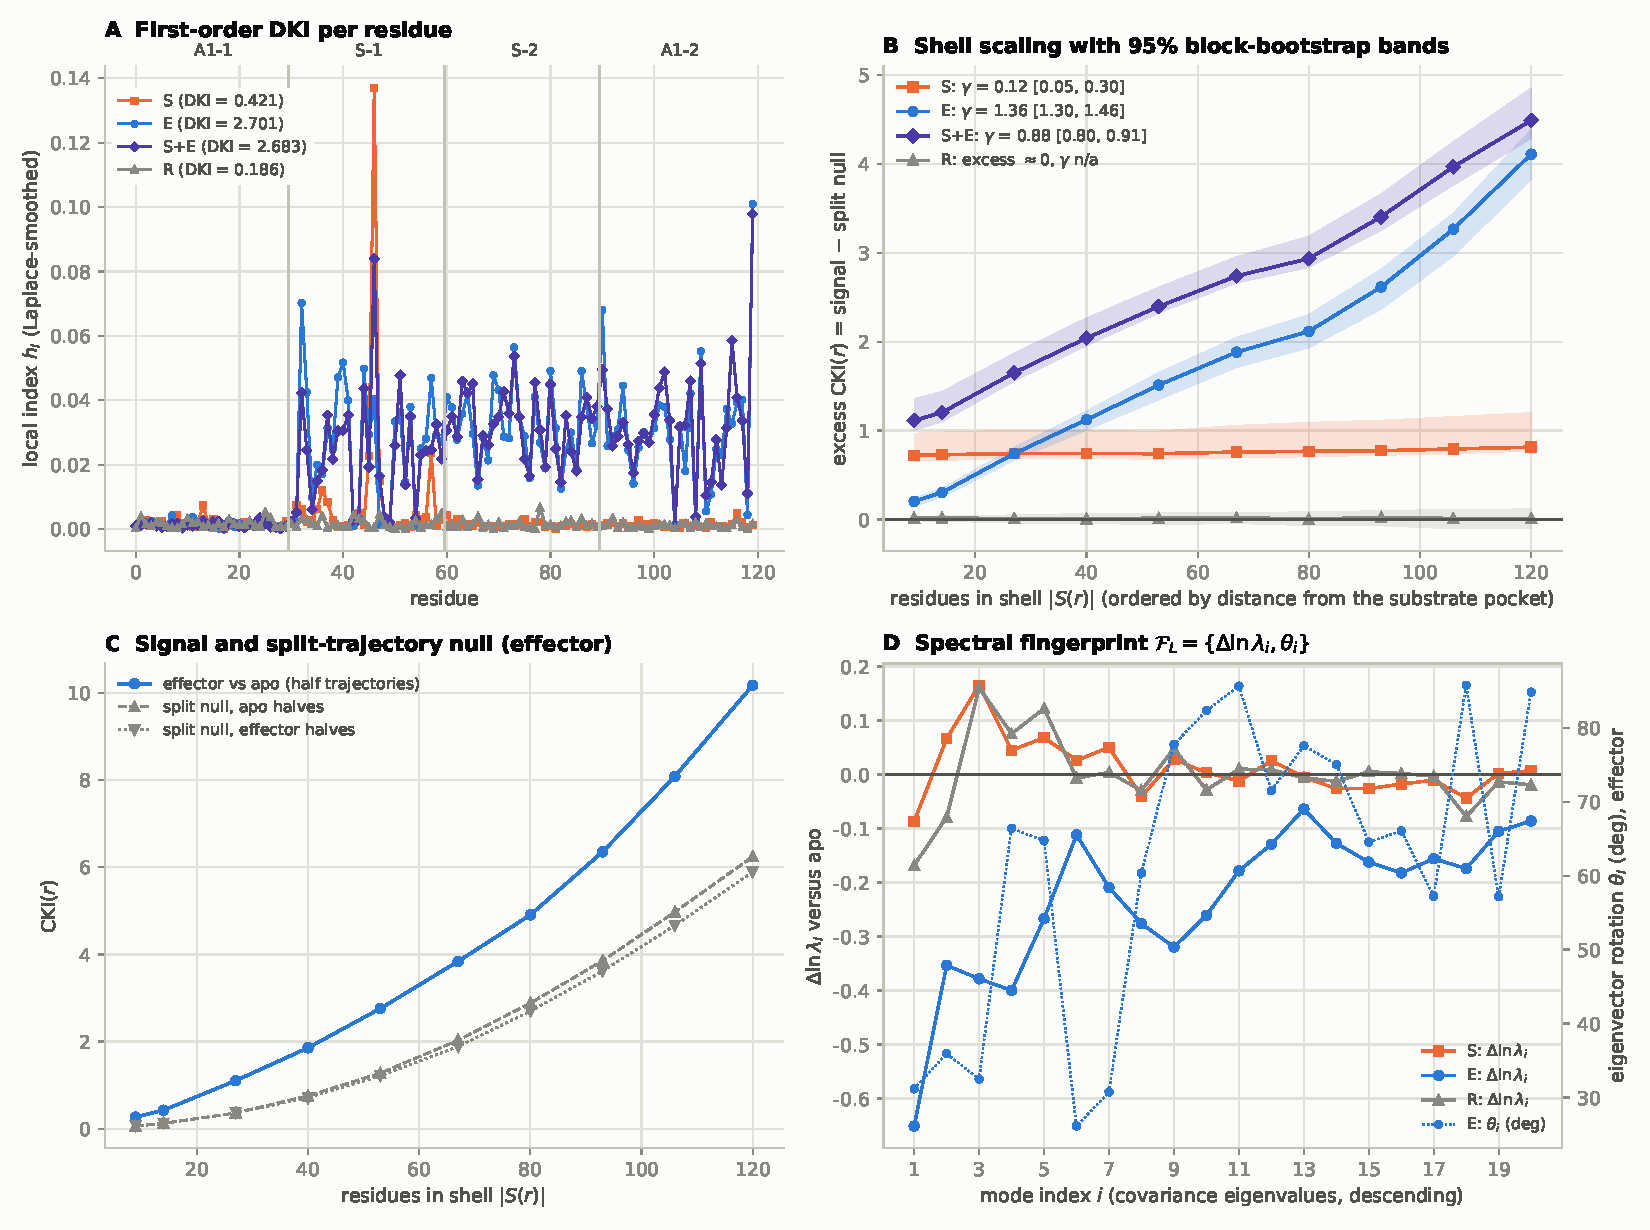
\includegraphics[width=\textwidth]{fig07_kakutani_diagnostics.pdf}
\caption{Diagnostics of the four-domain benchmark.
\textbf{A.} Local first-order index $h_i$ per residue for the substrate, effector and combined complexes and for the unliganded replica; the domain boundaries are marked. The substrate signal is a sharp peak in S-1, the effector signal extends over S-1, S-2 and A1-2.
\textbf{B.} Excess $\Delta\mathrm{CKI}(r)$ against the number of residues in the shell, with $95\%$ within-half block-bootstrap bands. The substrate curve is flat beyond the pocket, the effector curve grows across the protein, and the replica stays at $0$ (Theorem~\ref{thm:shell}).
\textbf{C.} Effector signal and the two split-trajectory null curves: the null carries the finite-sample bias, which grows with the dimension of the shell.
\textbf{D.} Spectral fingerprint: $\Delta\ln\lambda_i$ of the leading $20$ modes for substrate, effector and replica, and the eigenvector rotation angles $\theta_i$ of the effector complex. Only the effector shifts exceed the replica's scatter.}
\label{fig:diag}
\end{figure}

\begin{figure}[ht]
\centering
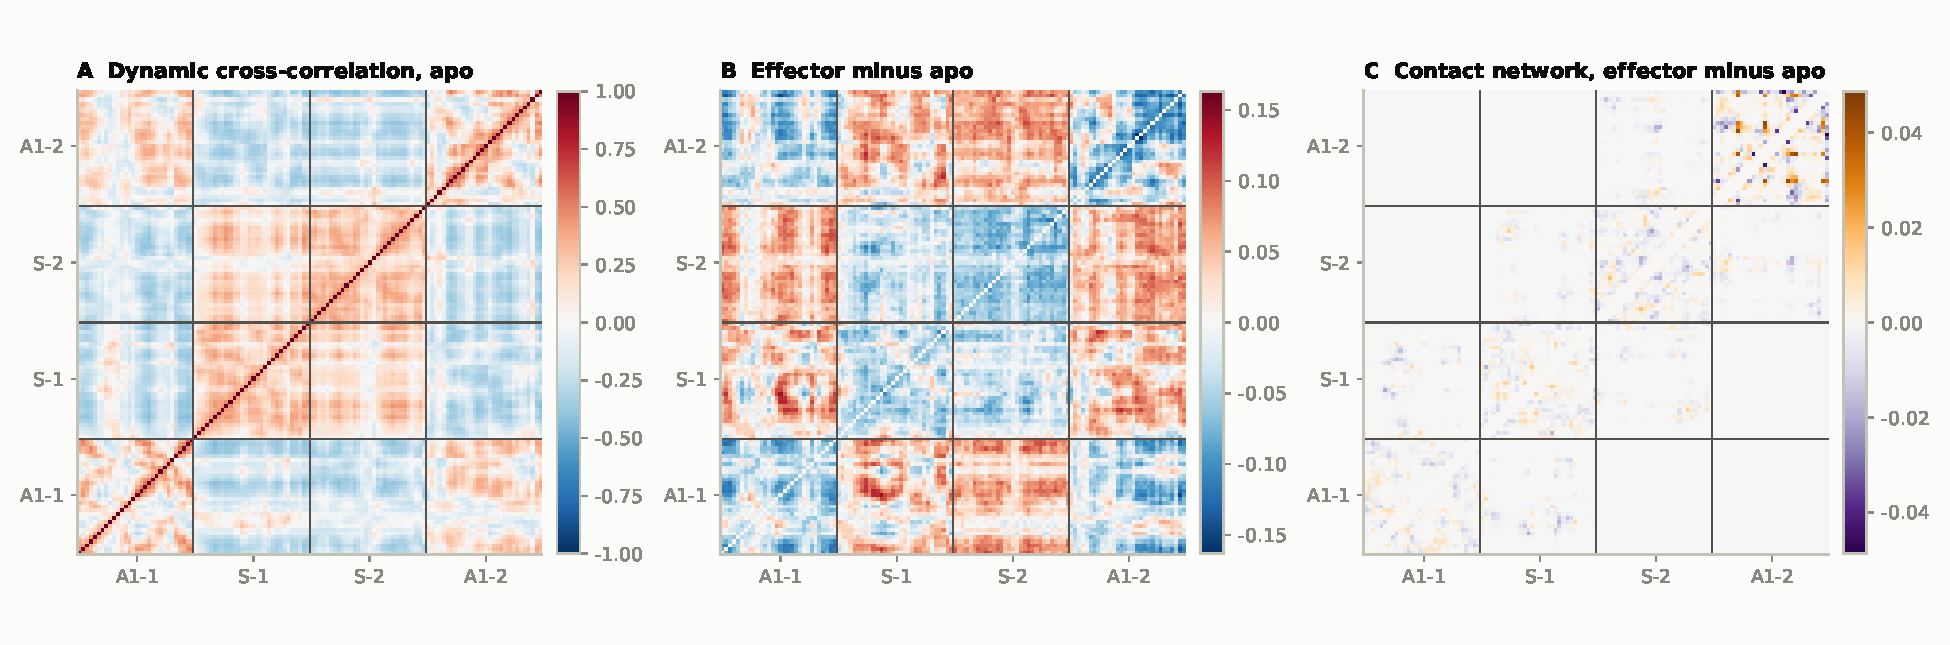
\includegraphics[width=\textwidth]{fig07_correlation_maps.pdf}
\caption{Correlation structure of the benchmark. \textbf{A.} Dynamic cross-correlation of the unliganded ensemble, with the four domains A1-1, S-1, S-2 and A1-2 marked. \textbf{B.} Change of the cross-correlation in the effector complex: the stiffened interfaces redistribute the correlations between all four domains. \textbf{C.} Change of the weighted contact network in the effector complex.}
\label{fig:maps}
\end{figure}

%%%%%%%%%%%%%%%%%%%%%%%%%%%%%%%%%%%%%%%%%%%%%%%%%%%%%%%%%%%%%%%%%%%%%%%%%%%%%%%
\clearpage
\section{Self-critical assessment, open problems, reproducibility and funding}
\label{sec:assessment}

We separate what is established from what is not.

\subsection*{Established}
\begin{itemize}[leftmargin=*]
\item The rigidity criterion and the count $\dim\ker H=12-\operatorname{rank}B$ for two rigid halves (Proposition~\ref{prop:rigidity}); the observed $11$ zero modes of the original geometry follow from it exactly.
\item Positivity of the Ledoit--Wolf estimate for any $T\ge2$, and the three-way decomposition with nonnegative terms (Theorem~\ref{thm:lw}).
\item Unbiasedness of the split-trajectory excess under the null hypothesis up to $O(\tau/h)$, and the cross-half leakage of resample-then-split bootstrapping (Theorem~\ref{thm:null}).
\item Monotonicity of the population shell curve and its plateau for perturbations confined to the pocket (Theorem~\ref{thm:shell}); by Corollary~\ref{cor:plateau} the population curve of the substrate model is exactly flat, including the rigid-body gauge.
\end{itemize}

\subsection*{Conditional or incomplete}
\begin{sloppypar}
\emph{(a) Synthetic data.} All benchmark results are obtained on synthetic trajectories of a coarse-grained $C_\alpha$ elastic network with known ground truth. The chain threading of the compact geometry contains virtual bonds up to $16$\,\AA, the dynamics are harmonic, and the dihedral chains are independent. The package has not yet been run on a real all-atom protein--ligand trajectory. There, anharmonic basins, coupled side chains and slow drift will stress the Gaussian approximation of the second-order index and the calibration of the null and the bootstrap.
\emph{(b) Input formats.} The native multi-model PDB reader is covered by the unit tests. The branch for DCD, XTC and other binary formats uses MDTraj \cite{McGibbon2015} and has not been executed, because MDTraj was not installed in the development environment.
\emph{(c) Interpretation limits.} The spectral fingerprint of the local substrate complex has log-eigenvalue shifts of the same size as those of the unliganded replica, about $\pm0.17$ on the leading modes, and is not interpreted. The distal exponent $\gamma$ is a log-log slope and is reported only when the excess interval excludes zero.
\emph{(d) Bootstrap calibration.} The intervals rest on $40$ replicates and have not been checked for coverage. The duplicate-frame bias (Proposition~\ref{prop:bias}) is corrected by a shift. This is a first-order correction, not a calibrated interval.
\end{sloppypar}

\subsection*{Relation to the literature}
The indices are the Kakutani affinity \cite{Kakutani1948} and the Bhattacharyya distance \cite{Bhattacharyya1943} in the forms developed in Papers~I--VI \cite{ChenChen2026I,ChenChen2026II,ChenChen2026III,ChenChen2026IV,ChenChen2026V,ChenChen2026VI} after the monograph \cite{Chen2026}. Covariance shrinkage is that of Ledoit and Wolf \cite{LedoitWolf2004}, cross-checked against \cite{Pedregosa2011}; the positivity of the rotation part rests on Fiedler's determinant inequality \cite{Fiedler1971}. The block bootstrap for dependent data is K\"unsch's \cite{Kunsch1989}, the bias correction follows \cite{EfronTibshirani1993}, and the autocorrelation window is Sokal's \cite{Sokal1997}. Superposition uses Kabsch's algorithm \cite{Kabsch1976}; the elastic network is that of \cite{Tirion1996,Atilgan2001}, and its rigidity analysis follows \cite{AsimowRoth1978}. Monotonicity under marginalisation is the data-processing inequality for $f$-divergences \cite{LieseVajda2006}. The ensemble view of allostery that motivates shell scaling is \cite{Motlagh2014}.

\begin{table}[ht]
\centering\small
\caption{Assessment of Paper VII.}
\label{tab:assessment}
\begin{tabular}{@{}>{\raggedright\arraybackslash}p{0.5\textwidth}>{\raggedright\arraybackslash}p{0.2\textwidth}>{\raggedright\arraybackslash}p{0.22\textwidth}@{}}
\toprule
Item & Status & Where \\
\midrule
$\dim\ker H=6$ criterion; $11=12-1$ for the loose geometry & established & Prop.~\ref{prop:rigidity}, Table~\ref{tab:rigidity} \\
Ledoit--Wolf positivity for $T<D$; three-way decomposition & established / verified & Thm.~\ref{thm:lw}, Table~\ref{tab:estimators} \\
Split-null excess; replica $3.10\to0.010$ & established / verified & Thm.~\ref{thm:null}, Table~\ref{tab:bootstrap} \\
Within-half bootstrap; duplicate-frame bias & established / verified & Thm.~\ref{thm:null}, Prop.~\ref{prop:bias} \\
Plateau of local perturbations, exact for the substrate model; $\gamma=0.12$, $1.36$, $0.88$ & established / verified & Thm.~\ref{thm:shell}, Cor.~\ref{cor:plateau}, Table~\ref{tab:scaling}(a), (b) \\
Real all-atom protein--ligand trajectories & open & Problem (1) \\
MDTraj input branch & untested & Section~6(b) \\
Coverage of the bootstrap intervals & open & Problem (2) \\
\bottomrule
\end{tabular}
\end{table}

\subsection*{Open problems}
\begin{enumerate}[label=(\arabic*),leftmargin=*]
\item \emph{Real trajectories.} Apply the pipeline to unliganded and liganded all-atom trajectories of a multi-domain allosteric enzyme with independent replicas, and test whether the replica excess is zero and the distal exponent separates orthosteric from allosteric ligands.
\item \emph{Coverage.} Measure the coverage of the percentile, bias-shifted and basic intervals on synthetic ensembles with known population index, as a function of the block length and the number of replicates.
\item \emph{Beyond Gaussian.} Replace the second-order index by a divergence between mixtures fitted to metastable basins, so that multimodal ensembles are not reduced to their covariance.
\item \emph{Block length.} Choose the block length from the autocorrelation of the index itself rather than of the leading principal component.
\end{enumerate}

\subsection*{Reproducibility}
{\raggedright
The package \texttt{kakutani\_pharma} (modules \texttt{featurizer}, \texttt{estimators}, \texttt{scaling}), its unit tests, the benchmark \texttt{benchmark\_allosteric\_protein.py} (about $16$ minutes) and the companion \texttt{code/paper07\_compute\_tables.py} use NumPy, SciPy and Matplotlib, with scikit-learn for the tests only. All random numbers derive from the seed $20260929$. The paper and its \LaTeX{} source (\texttt{paper/}), the data (\texttt{data/}), the figures (\texttt{figures/}) and the derived tables (\texttt{results/}) are archived under DOI \href{https://doi.org/10.5281/zenodo.23039869}{10.5281/zenodo.23039869} and maintained at \url{https://github.com/Ruqing1963/kakutani-statistical-pharmacology-VII}.\par}

\subsection*{Funding}
This project was supported by the National Natural Science Foundation of China (No.~22464010), the Guangxi Natural Science Foundation of China (No.~2025GXNSFAA069294), and the 2025 Bagui Youth Top Talent Project.

\begin{thebibliography}{99}
\bibitem{AsimowRoth1978} L.~Asimow and B.~Roth, \emph{The rigidity of graphs}, Trans. Amer. Math. Soc. \textbf{245} (1978), 279--289.
\bibitem{Atilgan2001} A.~R. Atilgan, S.~R. Durell, R.~L. Jernigan, M.~C. Demirel, O.~Keskin and I.~Bahar, \emph{Anisotropy of fluctuation dynamics of proteins with an elastic network model}, Biophys. J. \textbf{80} (2001), 505--515.
\bibitem{Bhattacharyya1943} A.~Bhattacharyya, \emph{On a measure of divergence between two statistical populations defined by their probability distributions}, Bull. Calcutta Math. Soc. \textbf{35} (1943), 99--109.
\bibitem{Chen2026} R.~Chen, \emph{Localized Bost--Connes systems}, assembled from the thirty-nine papers of the series, 2026, DOI 10.5281/zenodo.22883179.
\bibitem{ChenChen2026I} Z.~Chen and R.~Chen, \emph{Statistical pharmacology via Kakutani dichotomy I: the marginal drug Kakutani index and the $\alpha_c=1/2$ criticality theorem in high-dimensional conformational ensembles}, 2026, DOI 10.5281/zenodo.23005921 (version 1.1: 10.5281/zenodo.23018827).
\bibitem{ChenChen2026II} Z.~Chen and R.~Chen, \emph{Statistical pharmacology via Kakutani dichotomy II: the correlated Kakutani index, the 99.95\% covariance dominance theorem, and spectral fingerprints of cryptic allostery}, 2026, DOI 10.5281/zenodo.23012217.
\bibitem{ChenChen2026III} Z.~Chen and R.~Chen, \emph{Statistical pharmacology via Kakutani dichotomy III: spectral Kakutani--Feldman--H\'ajek criticality of correlated conformational modes: mode amplitude perturbation, iso-spectral Givens rotation, and tail-increment finite-size elimination}, 2026, DOI 10.5281/zenodo.23015709 (version 1.1: 10.5281/zenodo.23019056).
\bibitem{ChenChen2026IV} Z.~Chen and R.~Chen, \emph{Statistical pharmacology via Kakutani dichotomy IV: KMS inverse-temperature criticality $\beta_c=1$, pocket-to-distal tail allostery, and the four-quadrant ligand classification}, 2026, DOI 10.5281/zenodo.23018236.
\bibitem{ChenChen2026V} Z.~Chen and R.~Chen, \emph{Statistical pharmacology via Kakutani dichotomy V: the chemical obstruction group $\Xi_\beta^{\mathrm{drug}}(S)$, Borel--Cantelli tail order parameters, and the relative-entropy staircase}, 2026, DOI 10.5281/zenodo.23027704.
\bibitem{ChenChen2026VI} Z.~Chen and R.~Chen, \emph{Statistical pharmacology via Kakutani dichotomy VI: Wasserstein phase separation $W_1(\varphi_+,\varphi_-)$, the single-step scan barrier, and cone-geodesic collective moves}, 2026, DOI 10.5281/zenodo.23029360.
\bibitem{EfronTibshirani1993} B.~Efron and R.~J. Tibshirani, \emph{An Introduction to the Bootstrap}, Chapman \& Hall, New York, 1993.
\bibitem{Fiedler1971} M.~Fiedler, \emph{Bounds for the determinant of the sum of Hermitian matrices}, Proc. Amer. Math. Soc. \textbf{30} (1971), 27--31.
\bibitem{Kabsch1976} W.~Kabsch, \emph{A solution for the best rotation to relate two sets of vectors}, Acta Cryst. A \textbf{32} (1976), 922--923.
\bibitem{Kakutani1948} S.~Kakutani, \emph{On equivalence of infinite product measures}, Ann. of Math. (2) \textbf{49} (1948), 214--224.
\bibitem{Kunsch1989} H.~R. K\"unsch, \emph{The jackknife and the bootstrap for general stationary observations}, Ann. Statist. \textbf{17} (1989), 1217--1241.
\bibitem{LedoitWolf2004} O.~Ledoit and M.~Wolf, \emph{A well-conditioned estimator for large-dimensional covariance matrices}, J. Multivariate Anal. \textbf{88} (2004), 365--411.
\bibitem{LieseVajda2006} F.~Liese and I.~Vajda, \emph{On divergences and informations in statistics and information theory}, IEEE Trans. Inform. Theory \textbf{52} (2006), 4394--4412.
\bibitem{McGibbon2015} R.~T. McGibbon, K.~A. Beauchamp, M.~P. Harrigan, C.~Klein, J.~M. Swails, C.~X. Hern\'andez, C.~R. Schwantes, L.-P. Wang, T.~J. Lane and V.~S. Pande, \emph{MDTraj: a modern open library for the analysis of molecular dynamics trajectories}, Biophys. J. \textbf{109} (2015), 1528--1532.
\bibitem{Motlagh2014} H.~N. Motlagh, J.~O. Wrabl, J.~Li and V.~J. Hilser, \emph{The ensemble nature of allostery}, Nature \textbf{508} (2014), 331--339.
\bibitem{Pedregosa2011} F.~Pedregosa et al., \emph{Scikit-learn: machine learning in Python}, J. Mach. Learn. Res. \textbf{12} (2011), 2825--2830.
\bibitem{Sokal1997} A.~D. Sokal, \emph{Monte Carlo methods in statistical mechanics: foundations and new algorithms}, in: Functional Integration (Carg\`ese, 1996), NATO Adv. Sci. Inst. Ser. B Phys. \textbf{361}, Plenum, New York, 1997, 131--192.
\bibitem{Tirion1996} M.~M. Tirion, \emph{Large amplitude elastic motions in proteins from a single-parameter, atomic analysis}, Phys. Rev. Lett. \textbf{77} (1996), 1905--1908.
\end{thebibliography}

\end{document}
